\documentclass[10pt,twocolumn,letterpaper]{article}

\usepackage[margin=0.75in]{geometry}
\usepackage[T1]{fontenc}
\usepackage[utf8]{inputenc}
\usepackage{lmodern}
\usepackage{microtype}
\usepackage{graphicx}
\usepackage{hyperref}
\usepackage{amsmath,amssymb}
\usepackage{booktabs}
\usepackage{caption}
\usepackage{subcaption}
\usepackage{flushend}
\usepackage{xcolor}

\title{Robot Ping-Pong Control Under Physics Variation:\\
Domain Randomization and Residual Reinforcement Learning}
\author{
Julia Novick \and Jonathan Zhang \and Mayand Gulati \and Sagnik Biswas\\
UC Santa Barbara
}
\date{Winter 2026}

\begin{document}
\maketitle

\begin{abstract}
We study robust robot ping-pong control in simulation under uncertain physical parameters. Our controller stack combines (i) a hand-engineered finite state machine with inverse kinematics (FSM+IK) and (ii) a residual Soft Actor-Critic (SAC) policy that outputs bounded joint-space corrections. We compare nominal SAC training and domain-randomized SAC training against the FSM+IK baseline under both nominal and randomized evaluation physics. At 1M environment steps, nominal SAC attains the best absolute performance (482 mean hits under nominal physics; 328 under randomized physics), while robust SAC exhibits stronger relative robustness trends under perturbation (\(+48.5\%\) from nominal to randomized settings at 1M, versus \(-32.0\%\) for nominal SAC). We also report non-monotonic learning dynamics (a 750k performance dip followed by a 1M rebound), variance behavior, and failure modes. The project code is publicly available at \url{https://github.com/MG-05/ping-pong-domain-randomization}.
\end{abstract}

\section{Introduction}
Robotic table tennis requires coordinated, high-frequency motion with tight timing constraints and strong sensitivity to contact dynamics. Small mismatches in mass, friction, or restitution can significantly change ball trajectories and destabilize a policy that appears strong in a single nominal simulator setting. This motivates robust control strategies that preserve performance under physics variation.

Our project investigates a \emph{residual learning} design: a reliable, structured controller (FSM+IK) provides the core behavior, and an RL policy learns corrective residuals. This hybrid setup offers two practical benefits: (1) safer exploration and improved sample efficiency versus pure end-to-end RL, and (2) explicit compatibility with domain randomization to improve out-of-distribution (OOD) behavior.

The central question is: \emph{Can residual SAC improve rally performance while remaining robust under randomized physics?} We answer this with systematic evaluation across baselines, checkpoints (500k/750k/1M), and two evaluation conditions (nominal and randomized physics).

\section{Related Work}
Our method combines ideas from entropy-regularized deep RL, sim-to-real robustness, and hybrid control:
\begin{itemize}
    \item \textbf{Soft Actor-Critic (SAC).} SAC is an off-policy maximum-entropy actor-critic algorithm that is effective in continuous control and stabilizes exploration via entropy regularization~\cite{haarnoja2018sac}.
    \item \textbf{Domain Randomization.} Randomizing simulator parameters during training can reduce overfitting to a single simulator and improve transfer/generalization~\cite{tobin2017domainrand,peng2018sim2real}.
    \item \textbf{Residual Reinforcement Learning.} Residual RL augments a conventional controller with learned corrections, often improving data efficiency and stability in contact-rich tasks~\cite{johannink2019residualrl}.
\end{itemize}

\section{Methods}
\subsection{Task and Controller Stack}
We consider repeated paddle-ball rallies with a simulated KUKA iiwa + Schunk WSG + paddle + ball setup in Drake. The baseline policy is an FSM+IK controller that predicts intercept timing, solves IK for paddle placement, and executes strike/follow-through phases.

Residual SAC is layered on top of this baseline: at each control step, SAC outputs bounded action corrections that are added to baseline commands before execution.

\subsection{Formal Definitions}
Let \(H\) denote mean hits per episode over \(N\) episodes.
\begin{itemize}
    \item \textbf{Performance:} \(H\) (higher is better).
    \item \textbf{Degradation under perturbation:}
    \[
    \Delta(\%) = 100\cdot\frac{H_{\text{rand}} - H_{\text{nom}}}{H_{\text{nom}}}.
    \]
    \item \textbf{Consistency under perturbation:}
    \[
    \mathrm{CV}(\%) = 100\cdot \frac{\sigma_{\text{rand}}}{H_{\text{rand}}}.
    \]
\end{itemize}

\subsection{Training Setup}
We train two SAC variants for 1M timesteps each:
\begin{itemize}
    \item \textbf{Nominal SAC:} fixed nominal physics during training.
    \item \textbf{Robust SAC:} per-episode physics randomization during training.
\end{itemize}
Shared core settings: MLP policy \([256,256]\), learning rate \(3\times 10^{-4}\), batch size 256, replay buffer 100k, \(\gamma=0.99\), \(\tau=0.005\), control \(dt=0.01\,\mathrm{s}\), max 2000 steps/episode.

\subsection{Domain Randomization Distribution}
During robust training, we randomize key physical parameters each episode.

\begin{table}[t]
\centering
\caption{Domain randomization ranges used for robust training.}
\label{tab:dr_ranges}
\begin{tabular}{lcc}
\toprule
Parameter & Min & Max \\
\midrule
Ball mass (kg) & 0.002 & 0.0035 \\
Ball friction & 0.15 & 0.30 \\
Ball restitution & 0.85 & 0.95 \\
Paddle mass (kg) & 0.08 & 0.15 \\
Paddle friction & 0.20 & 0.60 \\
Paddle restitution & 0.80 & 1.00 \\
Floor dissipation & 0.01 & 0.10 \\
Floor restitution & 0.80 & 1.00 \\
\bottomrule
\end{tabular}
\end{table}

\subsection{Evaluation Protocol}
All policies are evaluated for 20 episodes per condition with deterministic policy inference. We report both nominal-physics and randomized-physics test conditions. To contextualize robustness, we also include FSM-only baseline evaluations from dedicated baseline reports.

\section{Results}
\subsection{Baseline Behavior}
The FSM+IK baseline is strong under deterministic nominal settings (159 deterministic hits in the 20-second horizon in the RL report; up to 154 hits in a separate baseline protocol with different initialization details). Under randomized starts/physics, baseline performance remains competitive but degrades relative to nominal, motivating learned residuals.

\subsection{Primary Quantitative Comparison}
Table~\ref{tab:main_results} summarizes the principal outcomes from the final evaluation JSON.

\begin{table*}[t]
\centering
\caption{Main comparison across models and evaluation physics (20 episodes/condition).}
\label{tab:main_results}
\begin{tabular}{lcccccc}
\toprule
Model & Eval Physics & Mean Hits & Std Hits & Max Hits & Mean Sim Time (s) & Degradation vs Nominal \\
\midrule
FSM Baseline & Nominal & 159.0 & 0.0 & 159 & 20.0 & -- \\
FSM Baseline & Randomized & 145.3 & 29.0 & 189 & 17.7 & \(-8.6\%\) \\
\midrule
Nominal SAC 500k & Nominal & 144.0 & 0.0 & 144 & 11.0 & -- \\
Nominal SAC 500k & Randomized & 112.8 & 55.1 & 274 & 8.5 & \(-21.7\%\) \\
Nominal SAC 750k & Nominal & 110.0 & 0.0 & 110 & 6.6 & -- \\
Nominal SAC 750k & Randomized & 61.3 & 35.9 & 156 & 3.9 & \(-44.3\%\) \\
Nominal SAC 1M & Nominal & \textbf{482.0} & 0.0 & \textbf{482} & 20.0 & -- \\
Nominal SAC 1M & Randomized & \textbf{328.0} & \textbf{106.0} & \textbf{474} & 13.9 & \(-32.0\%\) \\
\midrule
Robust SAC 500k & Nominal & 53.0 & 0.0 & 53 & 3.5 & -- \\
Robust SAC 500k & Randomized & 43.4 & 11.0 & 66 & 2.8 & \(-18.2\%\) \\
Robust SAC 750k & Nominal & 23.0 & 0.0 & 23 & 1.7 & -- \\
Robust SAC 750k & Randomized & 29.0 & 7.5 & 51 & 1.8 & \(+25.9\%\) \\
Robust SAC 1M & Nominal & 76.0 & 0.0 & 76 & 1.7 & -- \\
Robust SAC 1M & Randomized & 112.9 & 30.9 & 181 & 2.7 & \(+48.5\%\) \\
\bottomrule
\end{tabular}
\end{table*}

\subsection{Visual Analysis}
Figure~\ref{fig:all_results} provides the four key views used in our analysis:
\begin{itemize}
    \item learning curves versus budget (500k/750k/1M),
    \item degradation under physics perturbation,
    \item variance/consistency under randomization,
    \item survival-time comparison.
\end{itemize}

\begin{figure*}[t]
    \centering
    \begin{subfigure}[b]{0.48\textwidth}
        \centering
        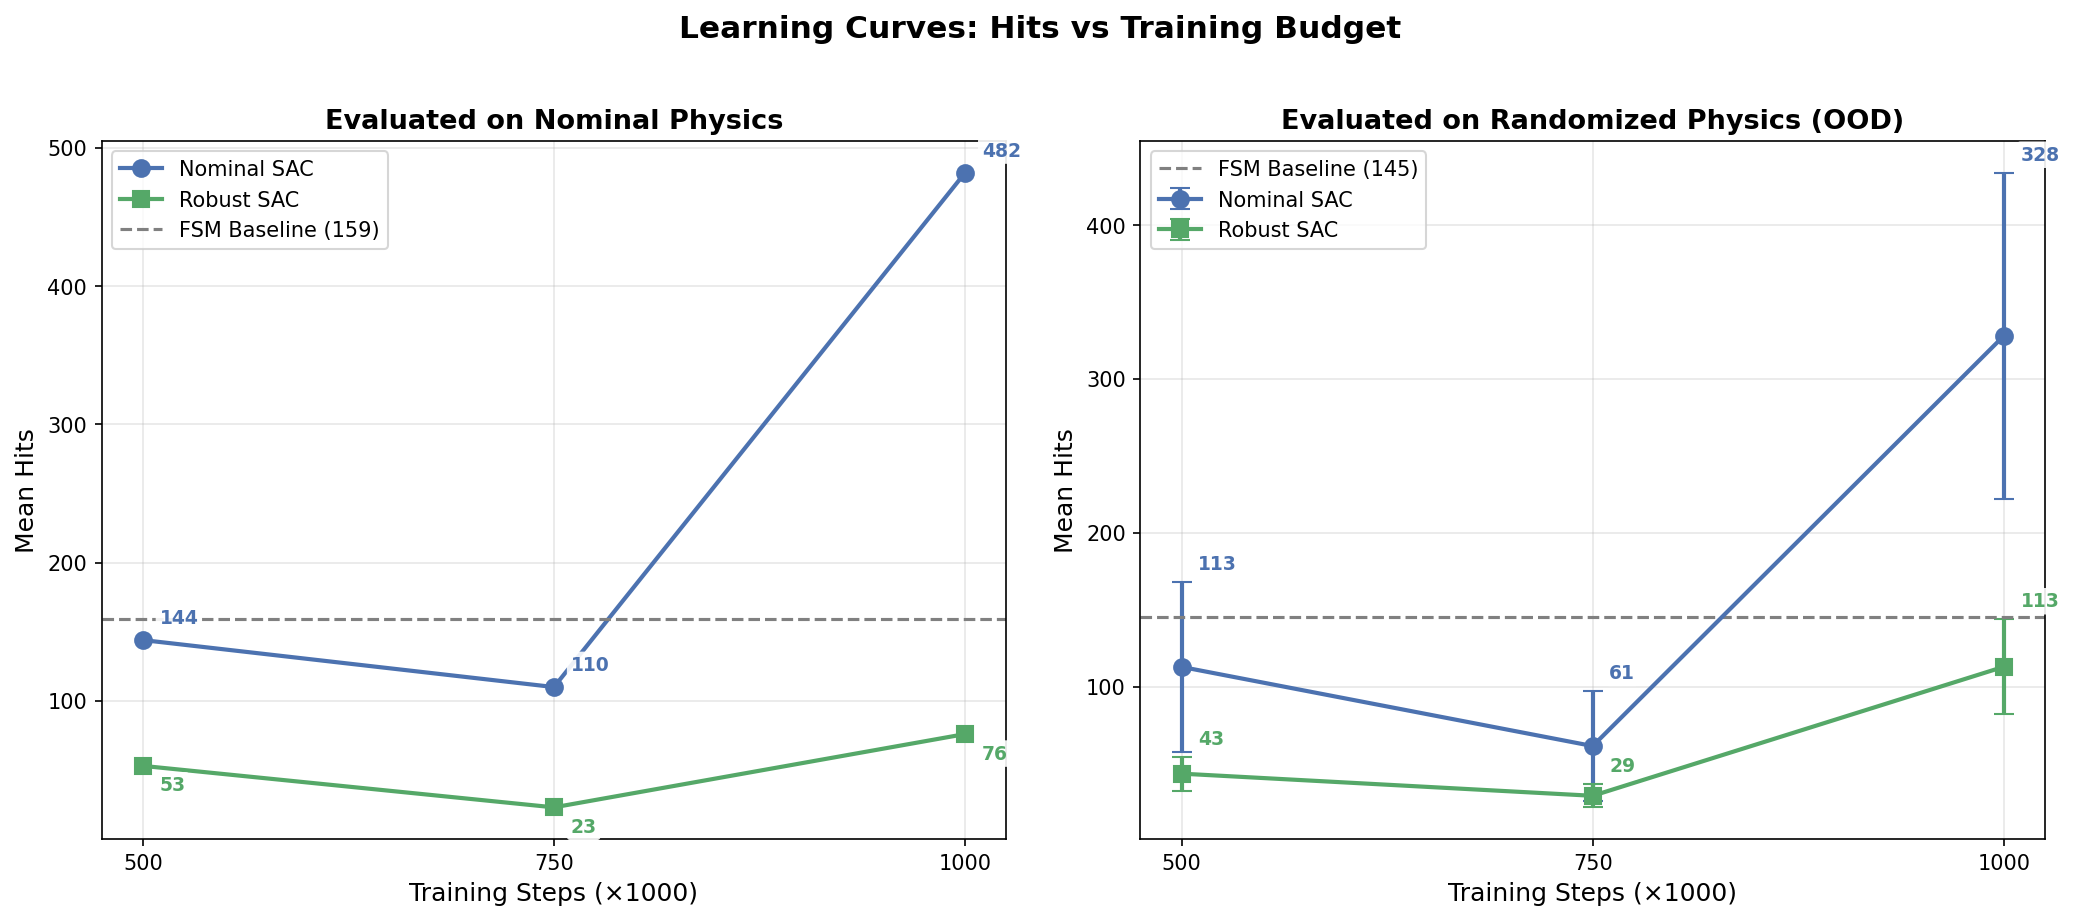
\includegraphics[width=\textwidth]{results/final_learning_curves.png}
        \caption{Learning curves over training budget.}
        \label{fig:learning_curves}
    \end{subfigure}
    \hfill
    \begin{subfigure}[b]{0.48\textwidth}
        \centering
        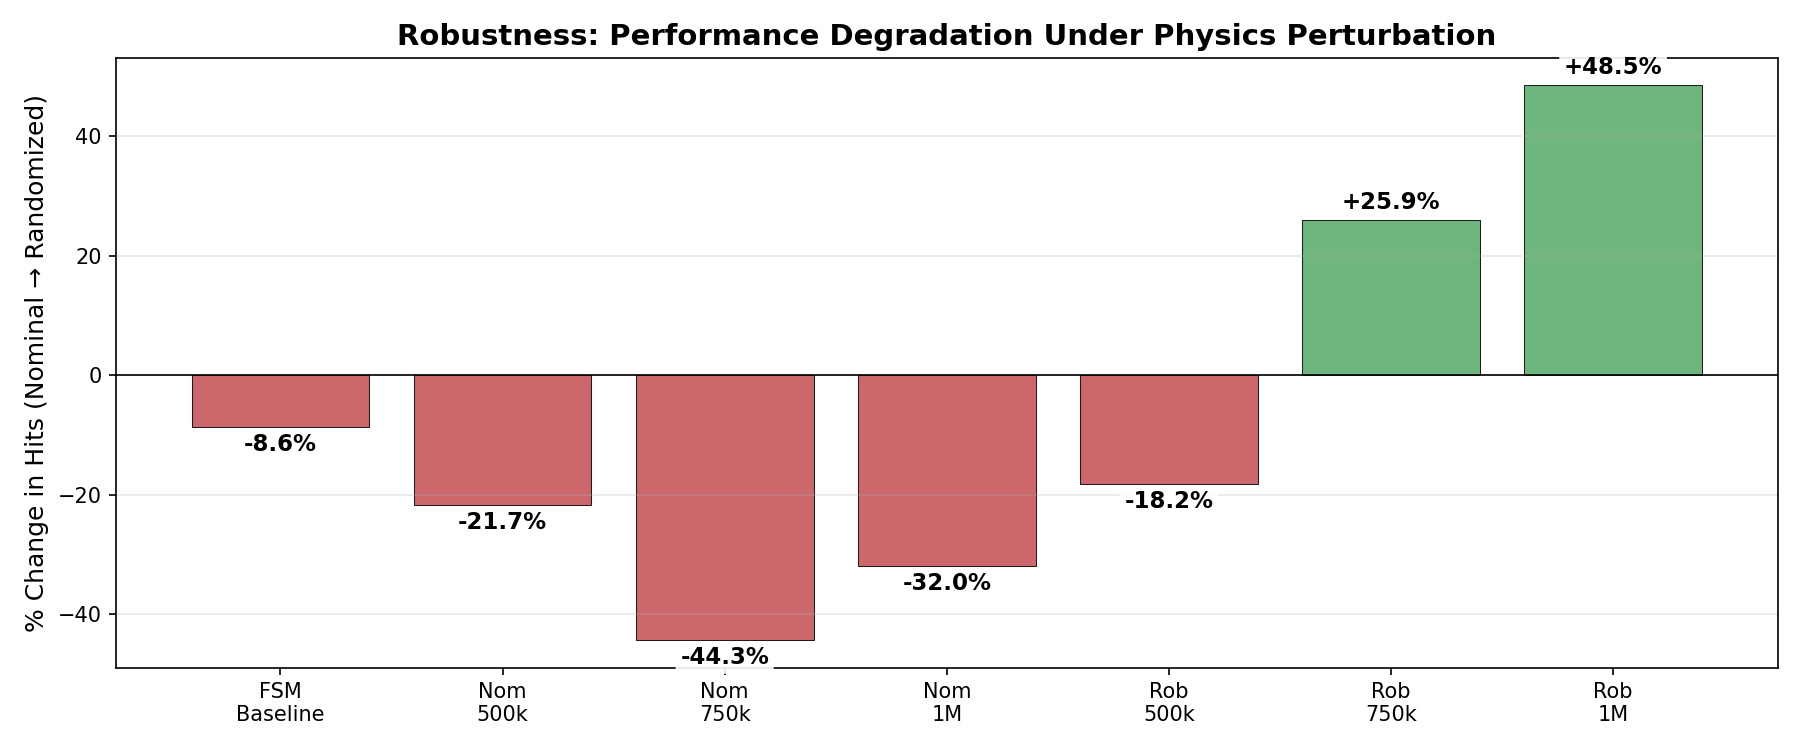
\includegraphics[width=\textwidth]{results/final_degradation.png}
        \caption{Relative degradation/improvement under randomized physics.}
        \label{fig:degradation}
    \end{subfigure}

    \vspace{0.4cm}
    \begin{subfigure}[b]{0.48\textwidth}
        \centering
        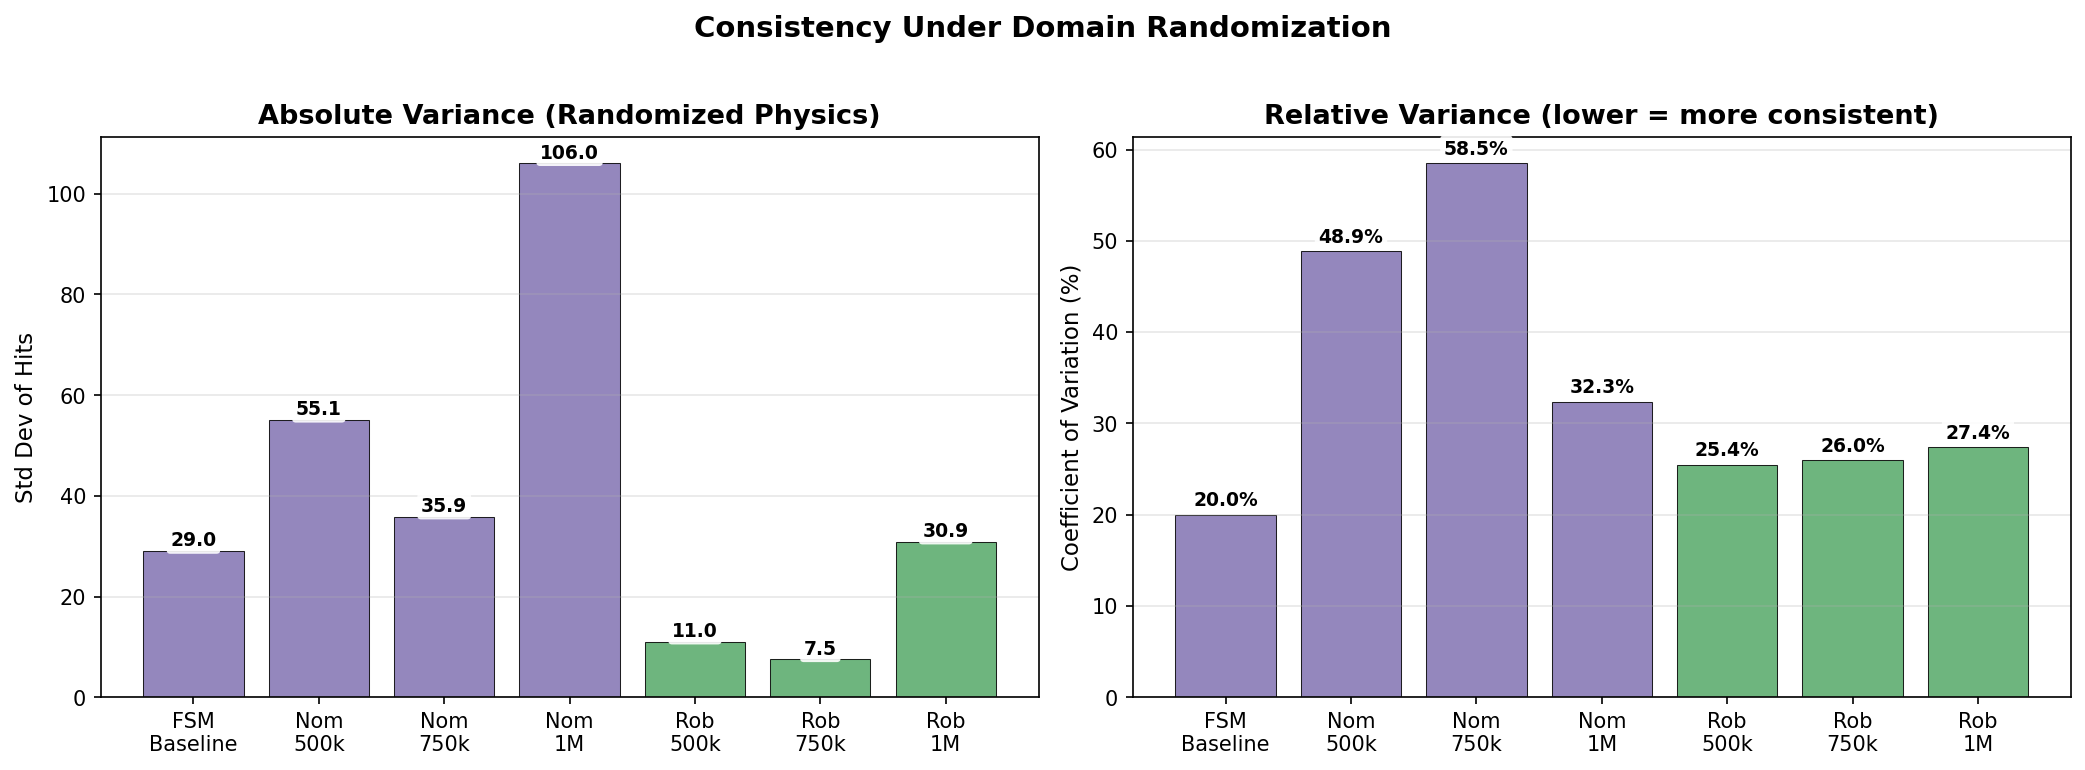
\includegraphics[width=\textwidth]{results/final_variance.png}
        \caption{Absolute and relative variability under randomization.}
        \label{fig:variance}
    \end{subfigure}
    \hfill
    \begin{subfigure}[b]{0.48\textwidth}
        \centering
        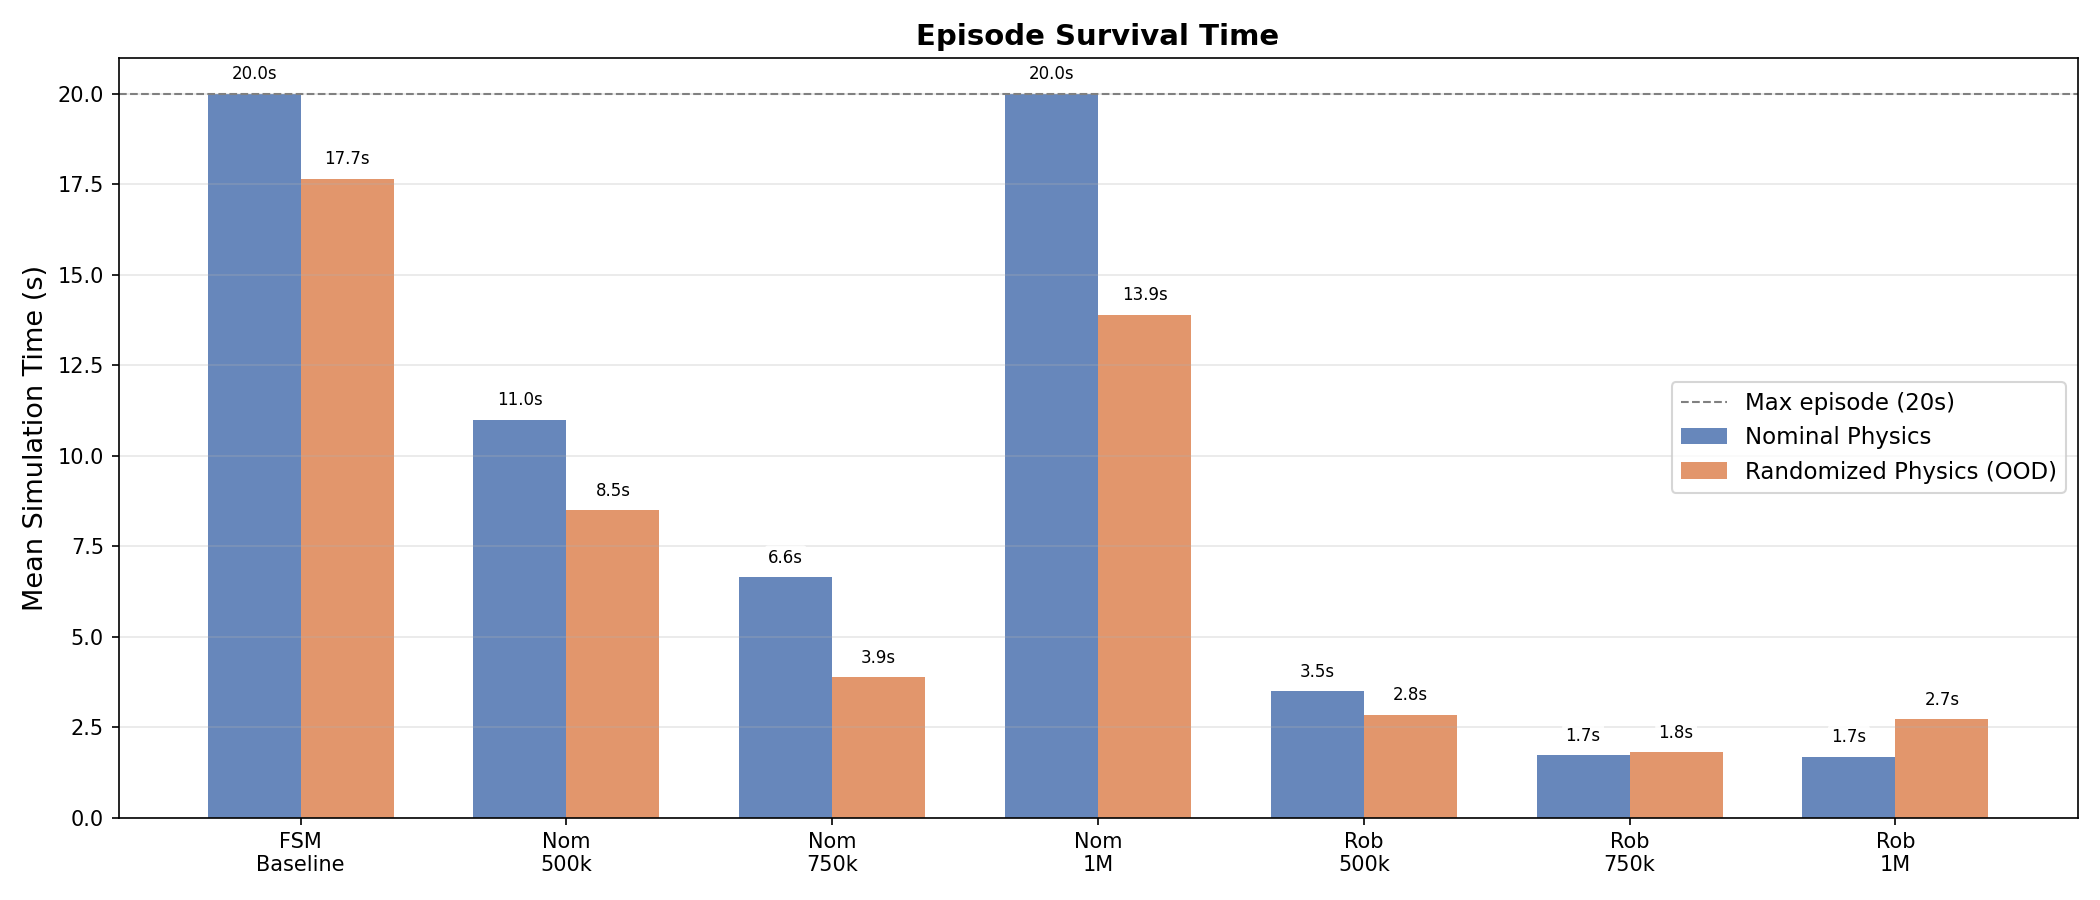
\includegraphics[width=\textwidth]{results/final_survival_time.png}
        \caption{Episode survival time comparison.}
        \label{fig:survival}
    \end{subfigure}
    \caption{Comprehensive evaluation of FSM baseline, nominal SAC, and robust SAC.}
    \label{fig:all_results}
\end{figure*}

\subsection{Key Findings}
\textbf{F1: Residual RL can dramatically improve peak performance.}
Nominal SAC at 1M reaches 482 mean hits under nominal physics, approximately \(3.0\times\) the baseline in this protocol.

\textbf{F2: Robustness trade-off is visible in relative metrics.}
Nominal SAC generally degrades under perturbation, while robust SAC (especially 750k/1M) improves under the randomized test distribution.

\textbf{F3: Learning is non-monotonic.}
Both nominal and robust tracks dip at 750k before recovering by 1M, underscoring the danger of early stopping conclusions.

\textbf{F4: Variance matters for deployment risk.}
Nominal SAC 1M has high OOD variance (\(\sigma=106\), CV \(=32.3\%\)); robust SAC 1M is lower-variance (CV \(=27.4\%\)) but lower in absolute peak hits.

\section{Discussion and Failure Analysis}
\subsection{What Worked}
The hybrid FSM+IK + residual SAC architecture successfully improved the baseline and revealed clear behavior differences between nominal-only and domain-randomized training.

\subsection{What Did Not Fully Work}
Our initial objective was to obtain a model that is simultaneously \emph{best in absolute performance} and \emph{best in robustness}. We only partially met this:
\begin{itemize}
    \item Nominal SAC achieved the highest hit counts but degraded under perturbation.
    \item Robust SAC improved relative robustness trends but did not match nominal SAC peak hit counts at 1M.
\end{itemize}
This negative/partial result is still informative: robust training appears to shift policy behavior toward consistency across a distribution, potentially at the cost of nominal specialization under the current training budget.

\subsection{Threats to Validity}
\begin{itemize}
    \item \textbf{Single-seed training runs:} limits confidence in statistical generalization.
    \item \textbf{Deterministic nominal evaluations:} some nominal standard deviations are near zero by construction.
    \item \textbf{Simulation-only evidence:} MuJoCo transfer scaffold exists, but full sim-to-real deployment was not completed.
\end{itemize}

\section{Conclusion}
We presented a residual RL approach for robot ping-pong under uncertain physics. A handcrafted FSM+IK controller provides a strong baseline, and residual SAC substantially boosts performance in favorable settings. Domain randomization materially changes OOD behavior, yielding improved relative robustness trends for robust SAC checkpoints even when absolute peak hits remain lower than nominal SAC. Overall, the project demonstrates a clear and sincere engineering/research effort with actionable insight into the peak-performance versus robustness trade-off.

\section*{Code Availability}
All code, reports, evaluation scripts, and generated plots are publicly available at:
\url{https://github.com/MG-05/ping-pong-domain-randomization}

\section*{Reproducibility}
Representative commands used for the presented artifacts:
\begin{verbatim}
python -m src.train_rl --steps 1000000 --no-randomize \
  --save-path data/sac_nominal_1m --seed 42
python -m src.train_rl --steps 1000000 --randomize \
  --save-path data/sac_robust_1m --seed 42
python scripts/run_all_evals.py
python results/generate_final_report.py
\end{verbatim}

\begin{thebibliography}{9}

\bibitem{haarnoja2018sac}
Tuomas Haarnoja, Aurick Zhou, Pieter Abbeel, and Sergey Levine.
\newblock Soft Actor-Critic: Off-Policy Maximum Entropy Deep Reinforcement Learning with a Stochastic Actor.
\newblock In \emph{ICML}, 2018.

\bibitem{tobin2017domainrand}
Josh Tobin, Rachel Fong, Alex Ray, Jonas Schneider, Wojciech Zaremba, and Pieter Abbeel.
\newblock Domain Randomization for Transferring Deep Neural Networks from Simulation to the Real World.
\newblock In \emph{IROS}, 2017.

\bibitem{peng2018sim2real}
Xue Bin Peng, Marcin Andrychowicz, Wojciech Zaremba, and Pieter Abbeel.
\newblock Sim-to-Real Transfer of Robotic Control with Dynamics Randomization.
\newblock In \emph{ICRA}, 2018.

\bibitem{johannink2019residualrl}
Tobias Johannink, Shikhar Bahl, Ashvin Nair, et al.
\newblock Residual Reinforcement Learning for Robot Control.
\newblock In \emph{ICRA}, 2019.

\end{thebibliography}

\end{document}
